Having successfully stabilised prototype bicycle...

\begin{figure}[H]
	\begin{subfigure}{0.475\textwidth}
	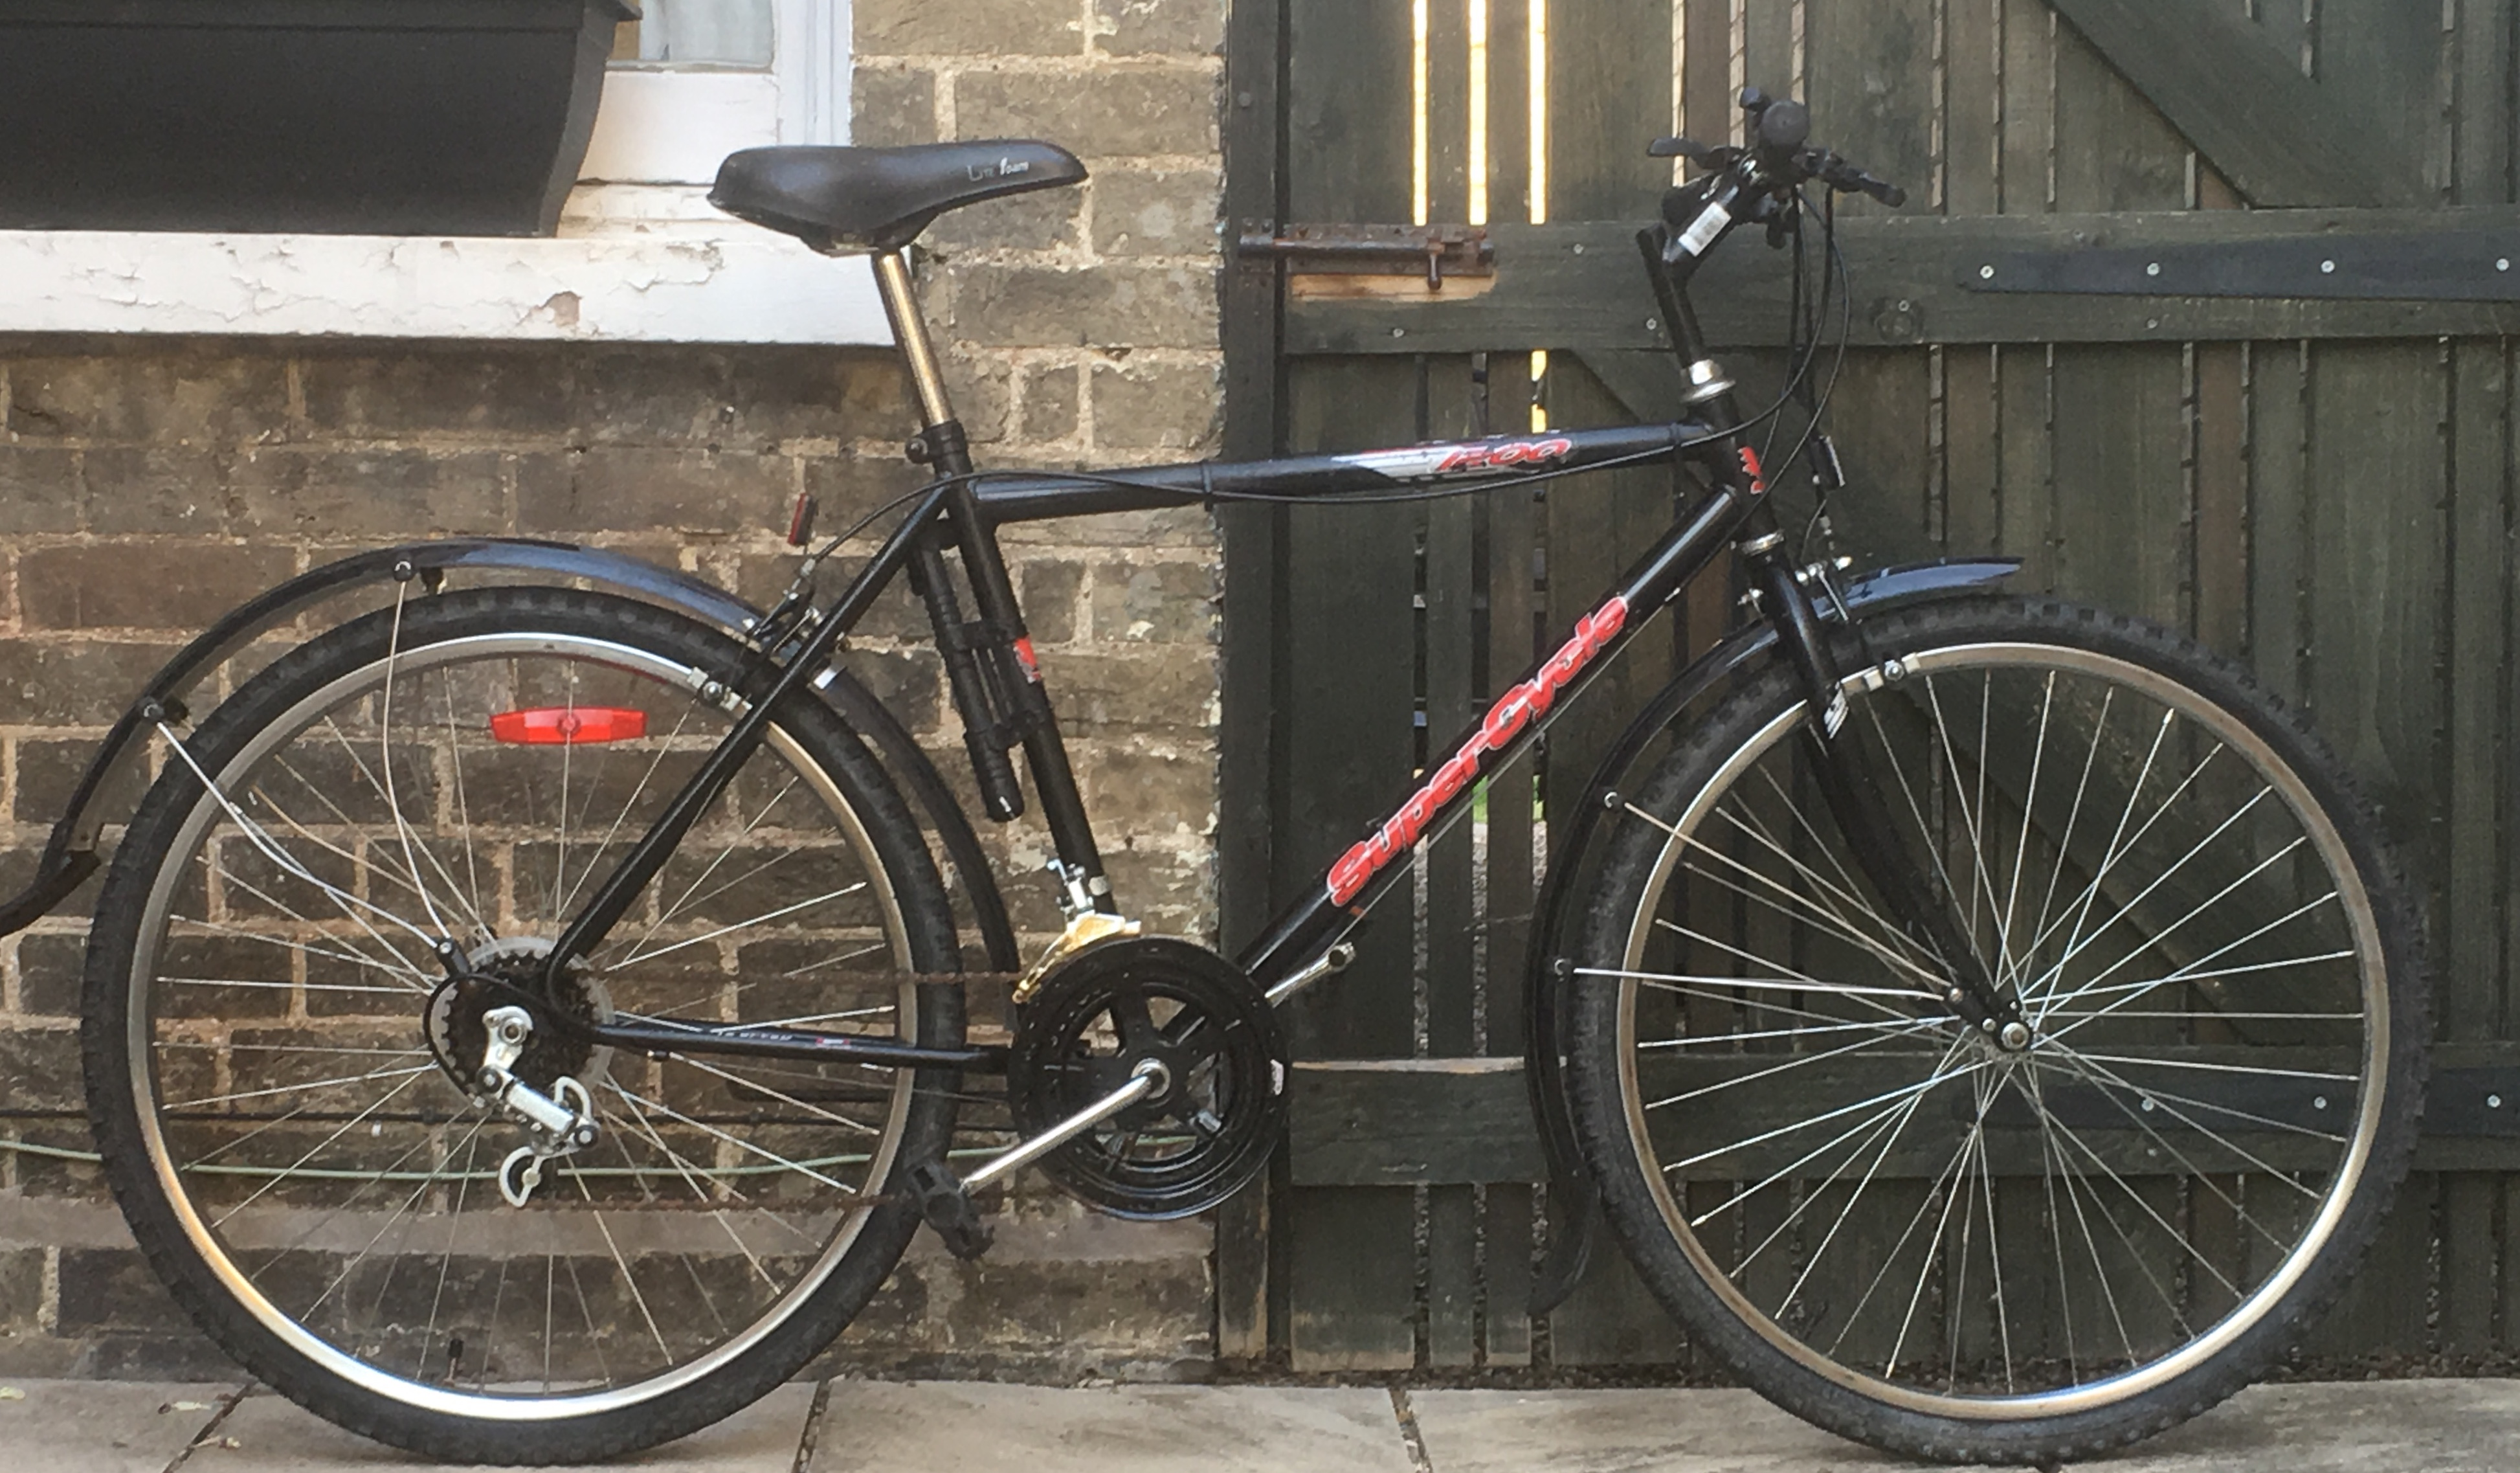
\includegraphics[scale=0.06]{FSBike}
	\caption{Unmodified Form}
	\end{subfigure} \hfill
	\begin{subfigure}{0.475\textwidth}
	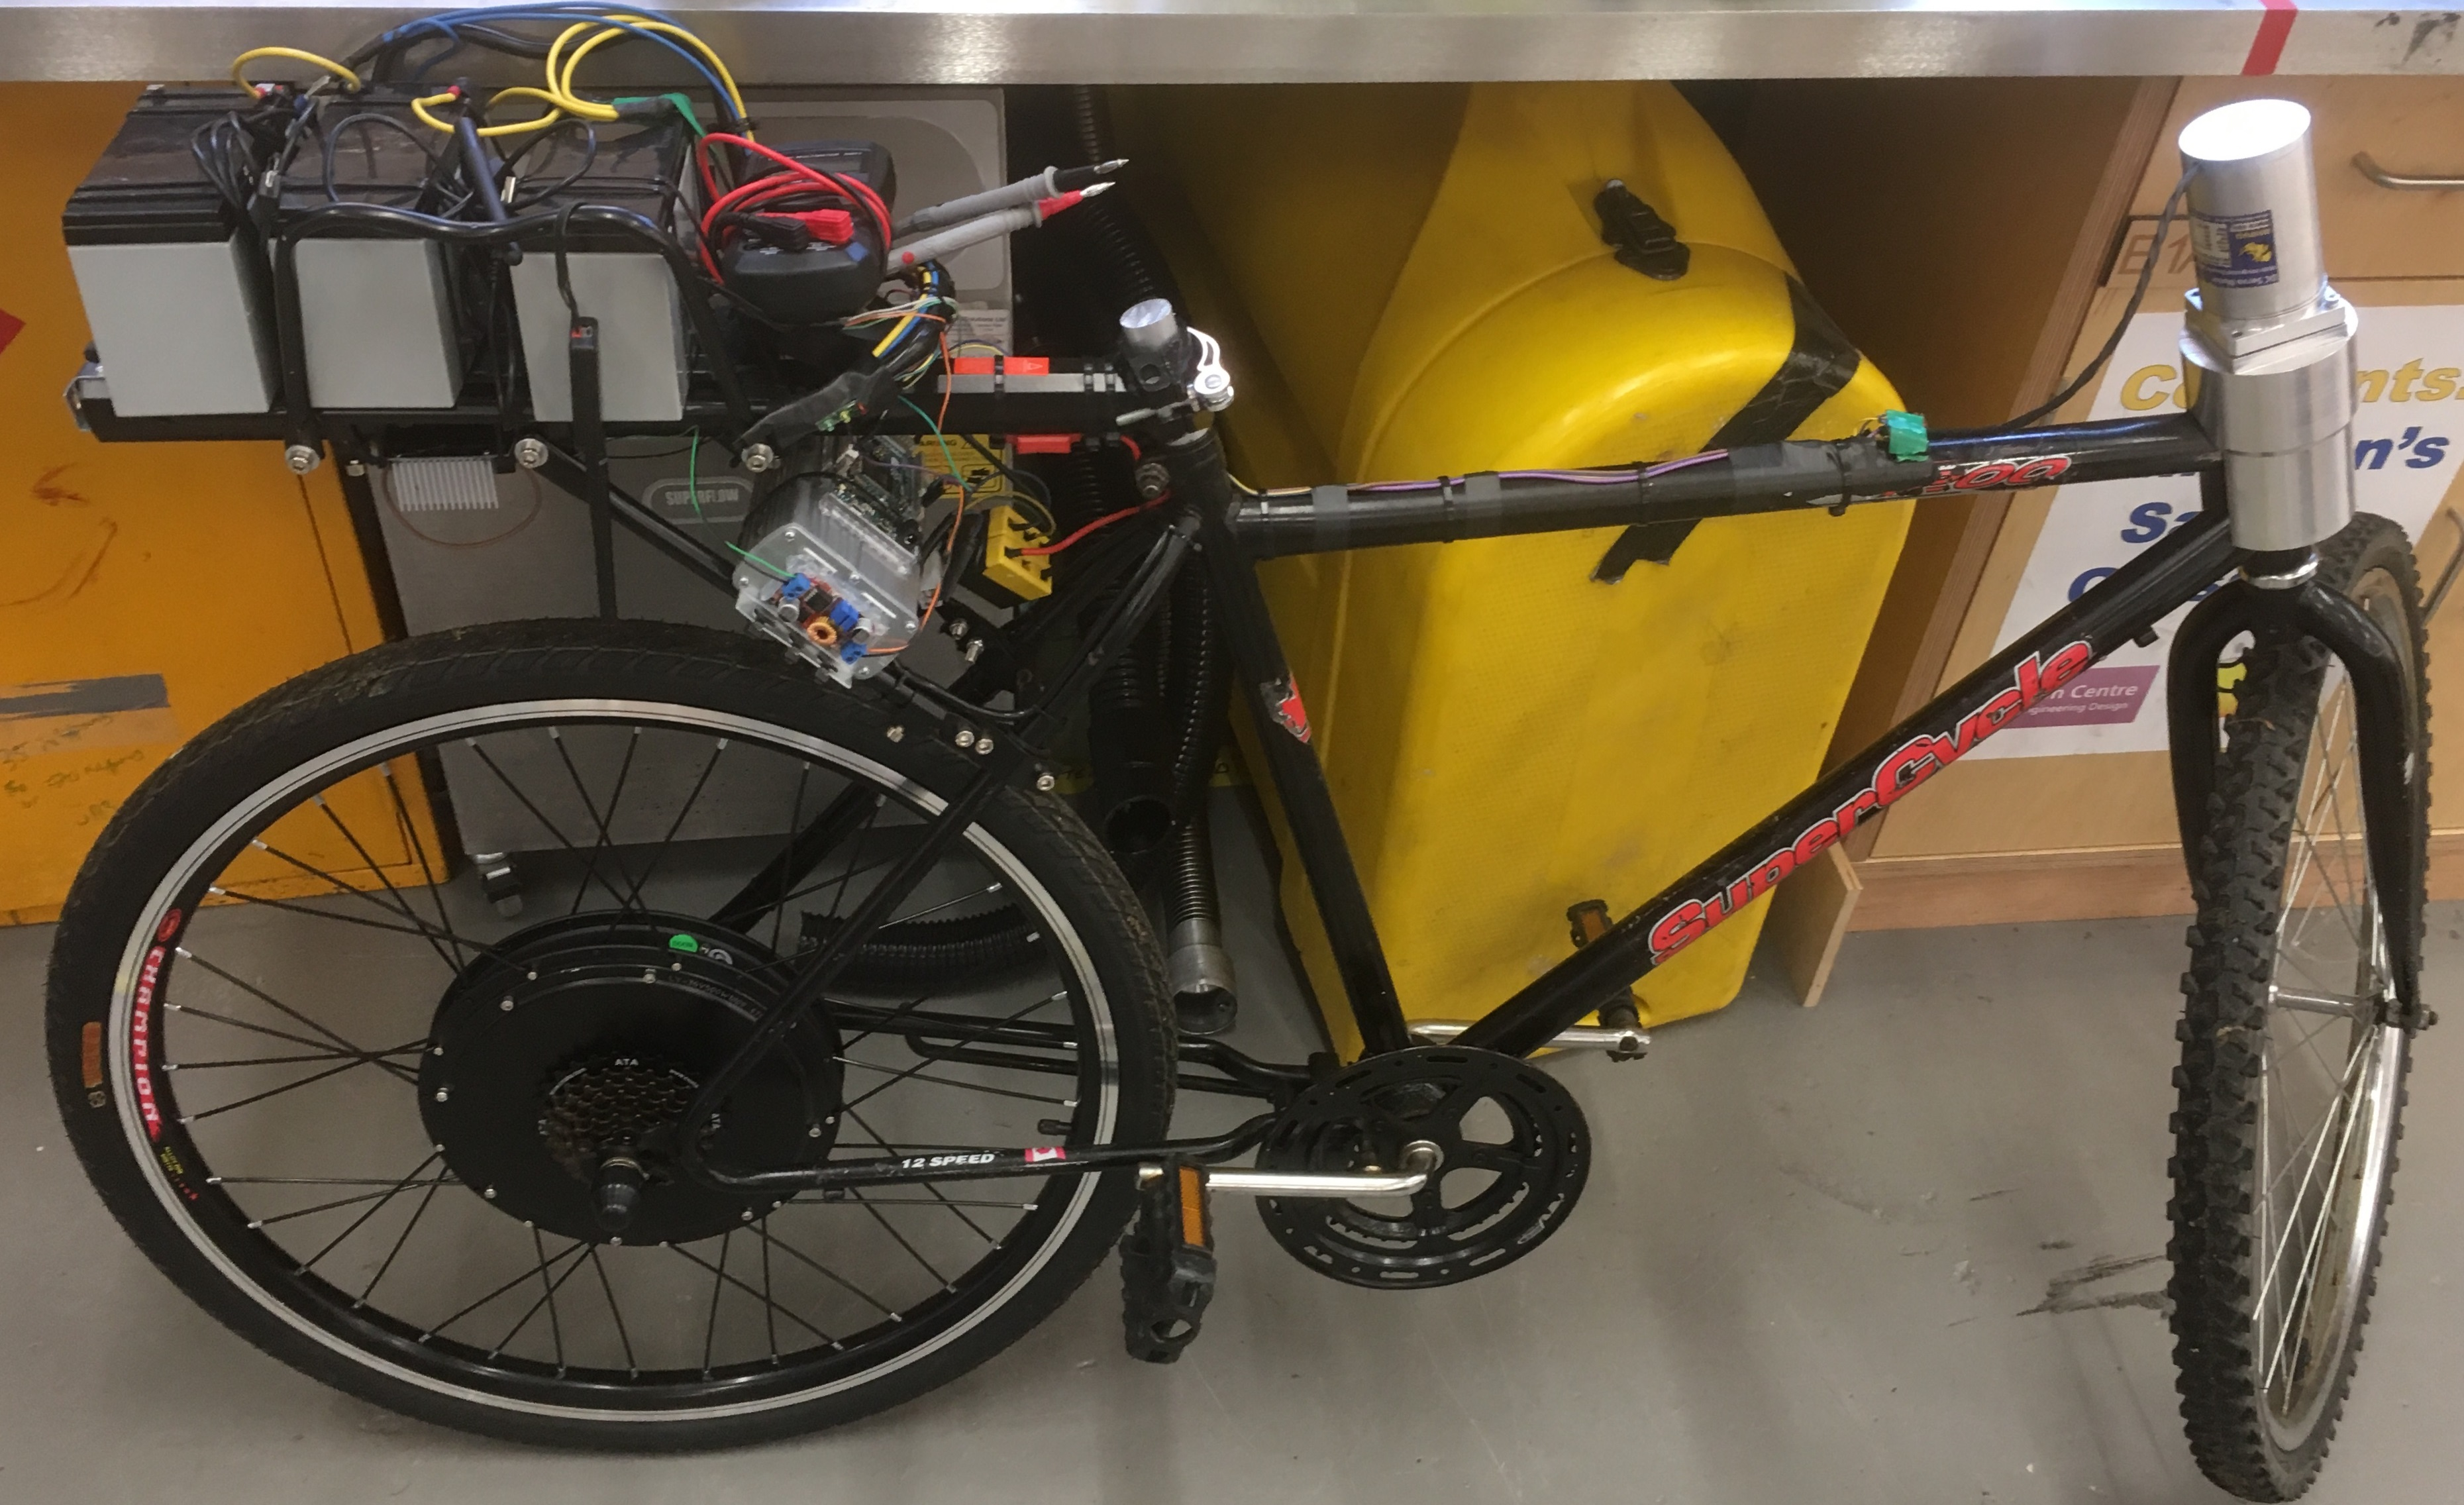
\includegraphics[scale=0.06]{FSBikeMod}
	\caption{After Modification}
	\end{subfigure}
	\caption{Full-Scale Bicycle Before and After Modification}
\end{figure}

\subsection{Hardware}

Arduino (32-bit instead of 8-bit) as controller, why particular servo, servo mounting design, battery, voltage regulators, drive motor, motor controller disassembly, etc. 

\newpage
\begin{figure}[H]
	\centering
	\begin{subfigure}[t]{0.475\textwidth}
		\centering
		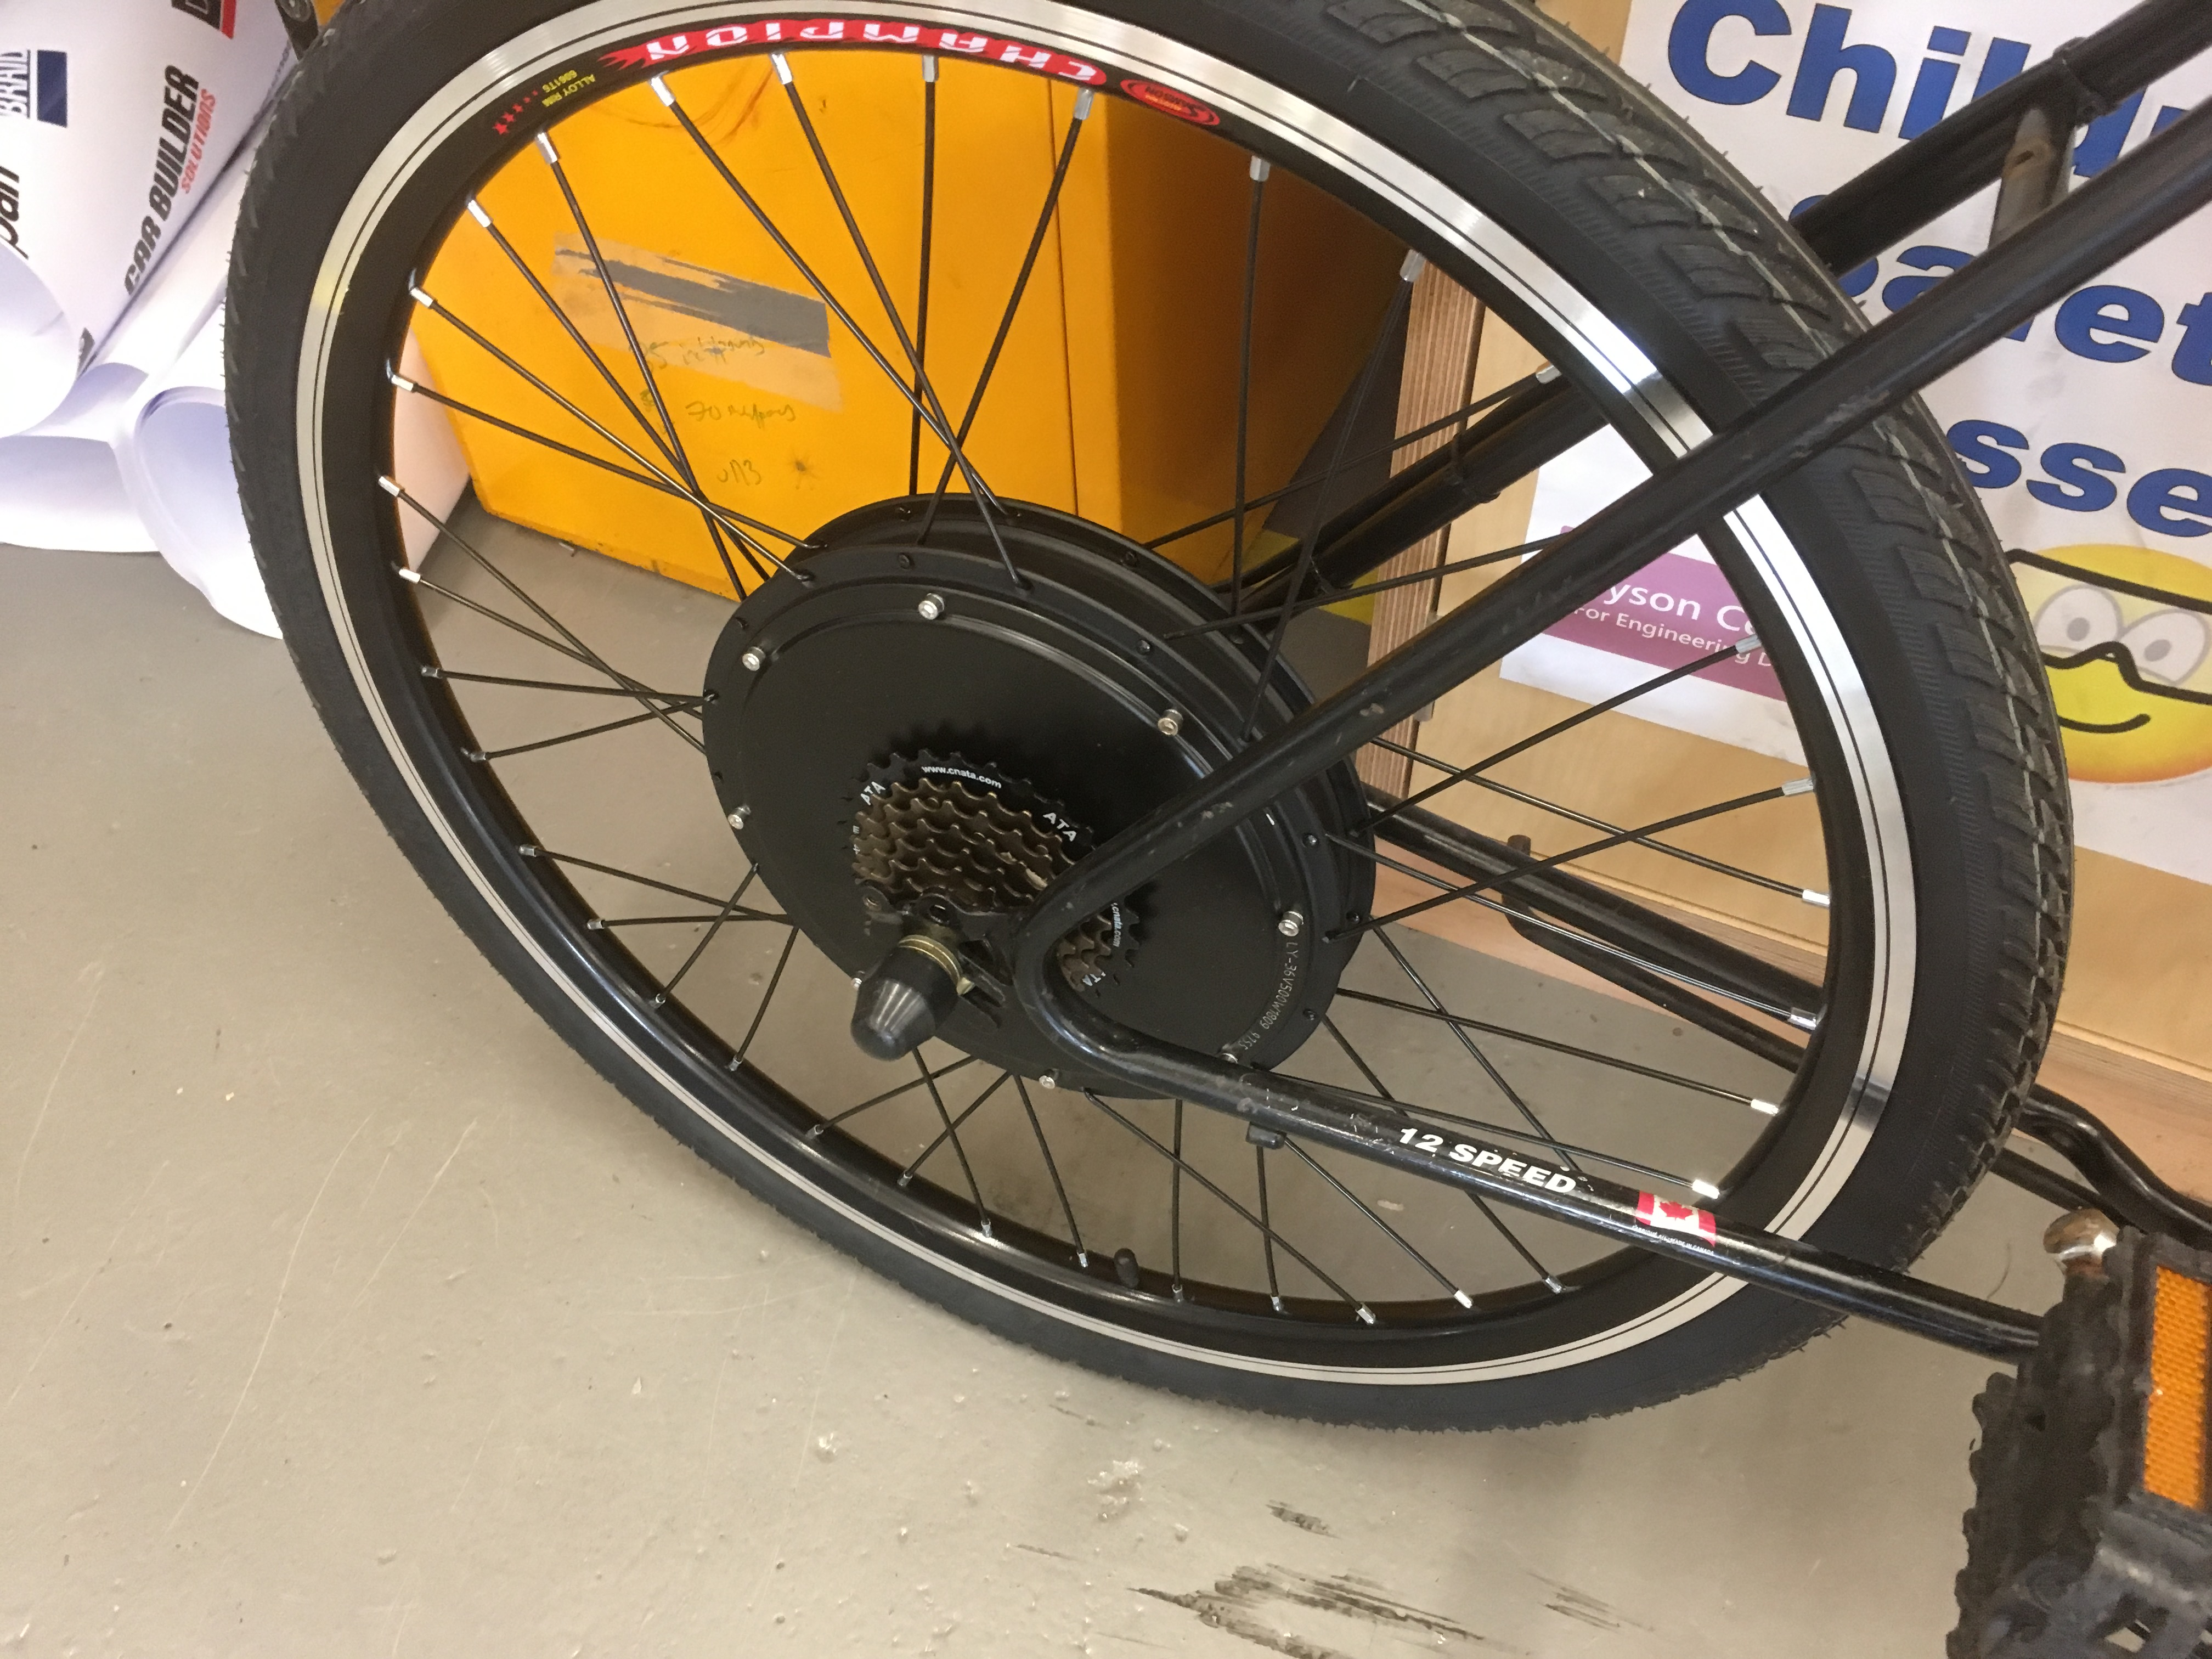
\includegraphics[width=\textwidth]{fsDrive}
		\caption{Rear Drive Motor}
		\end{subfigure}
	\hfill
	\begin{subfigure}[t]{0.475\textwidth}  
		\centering 
		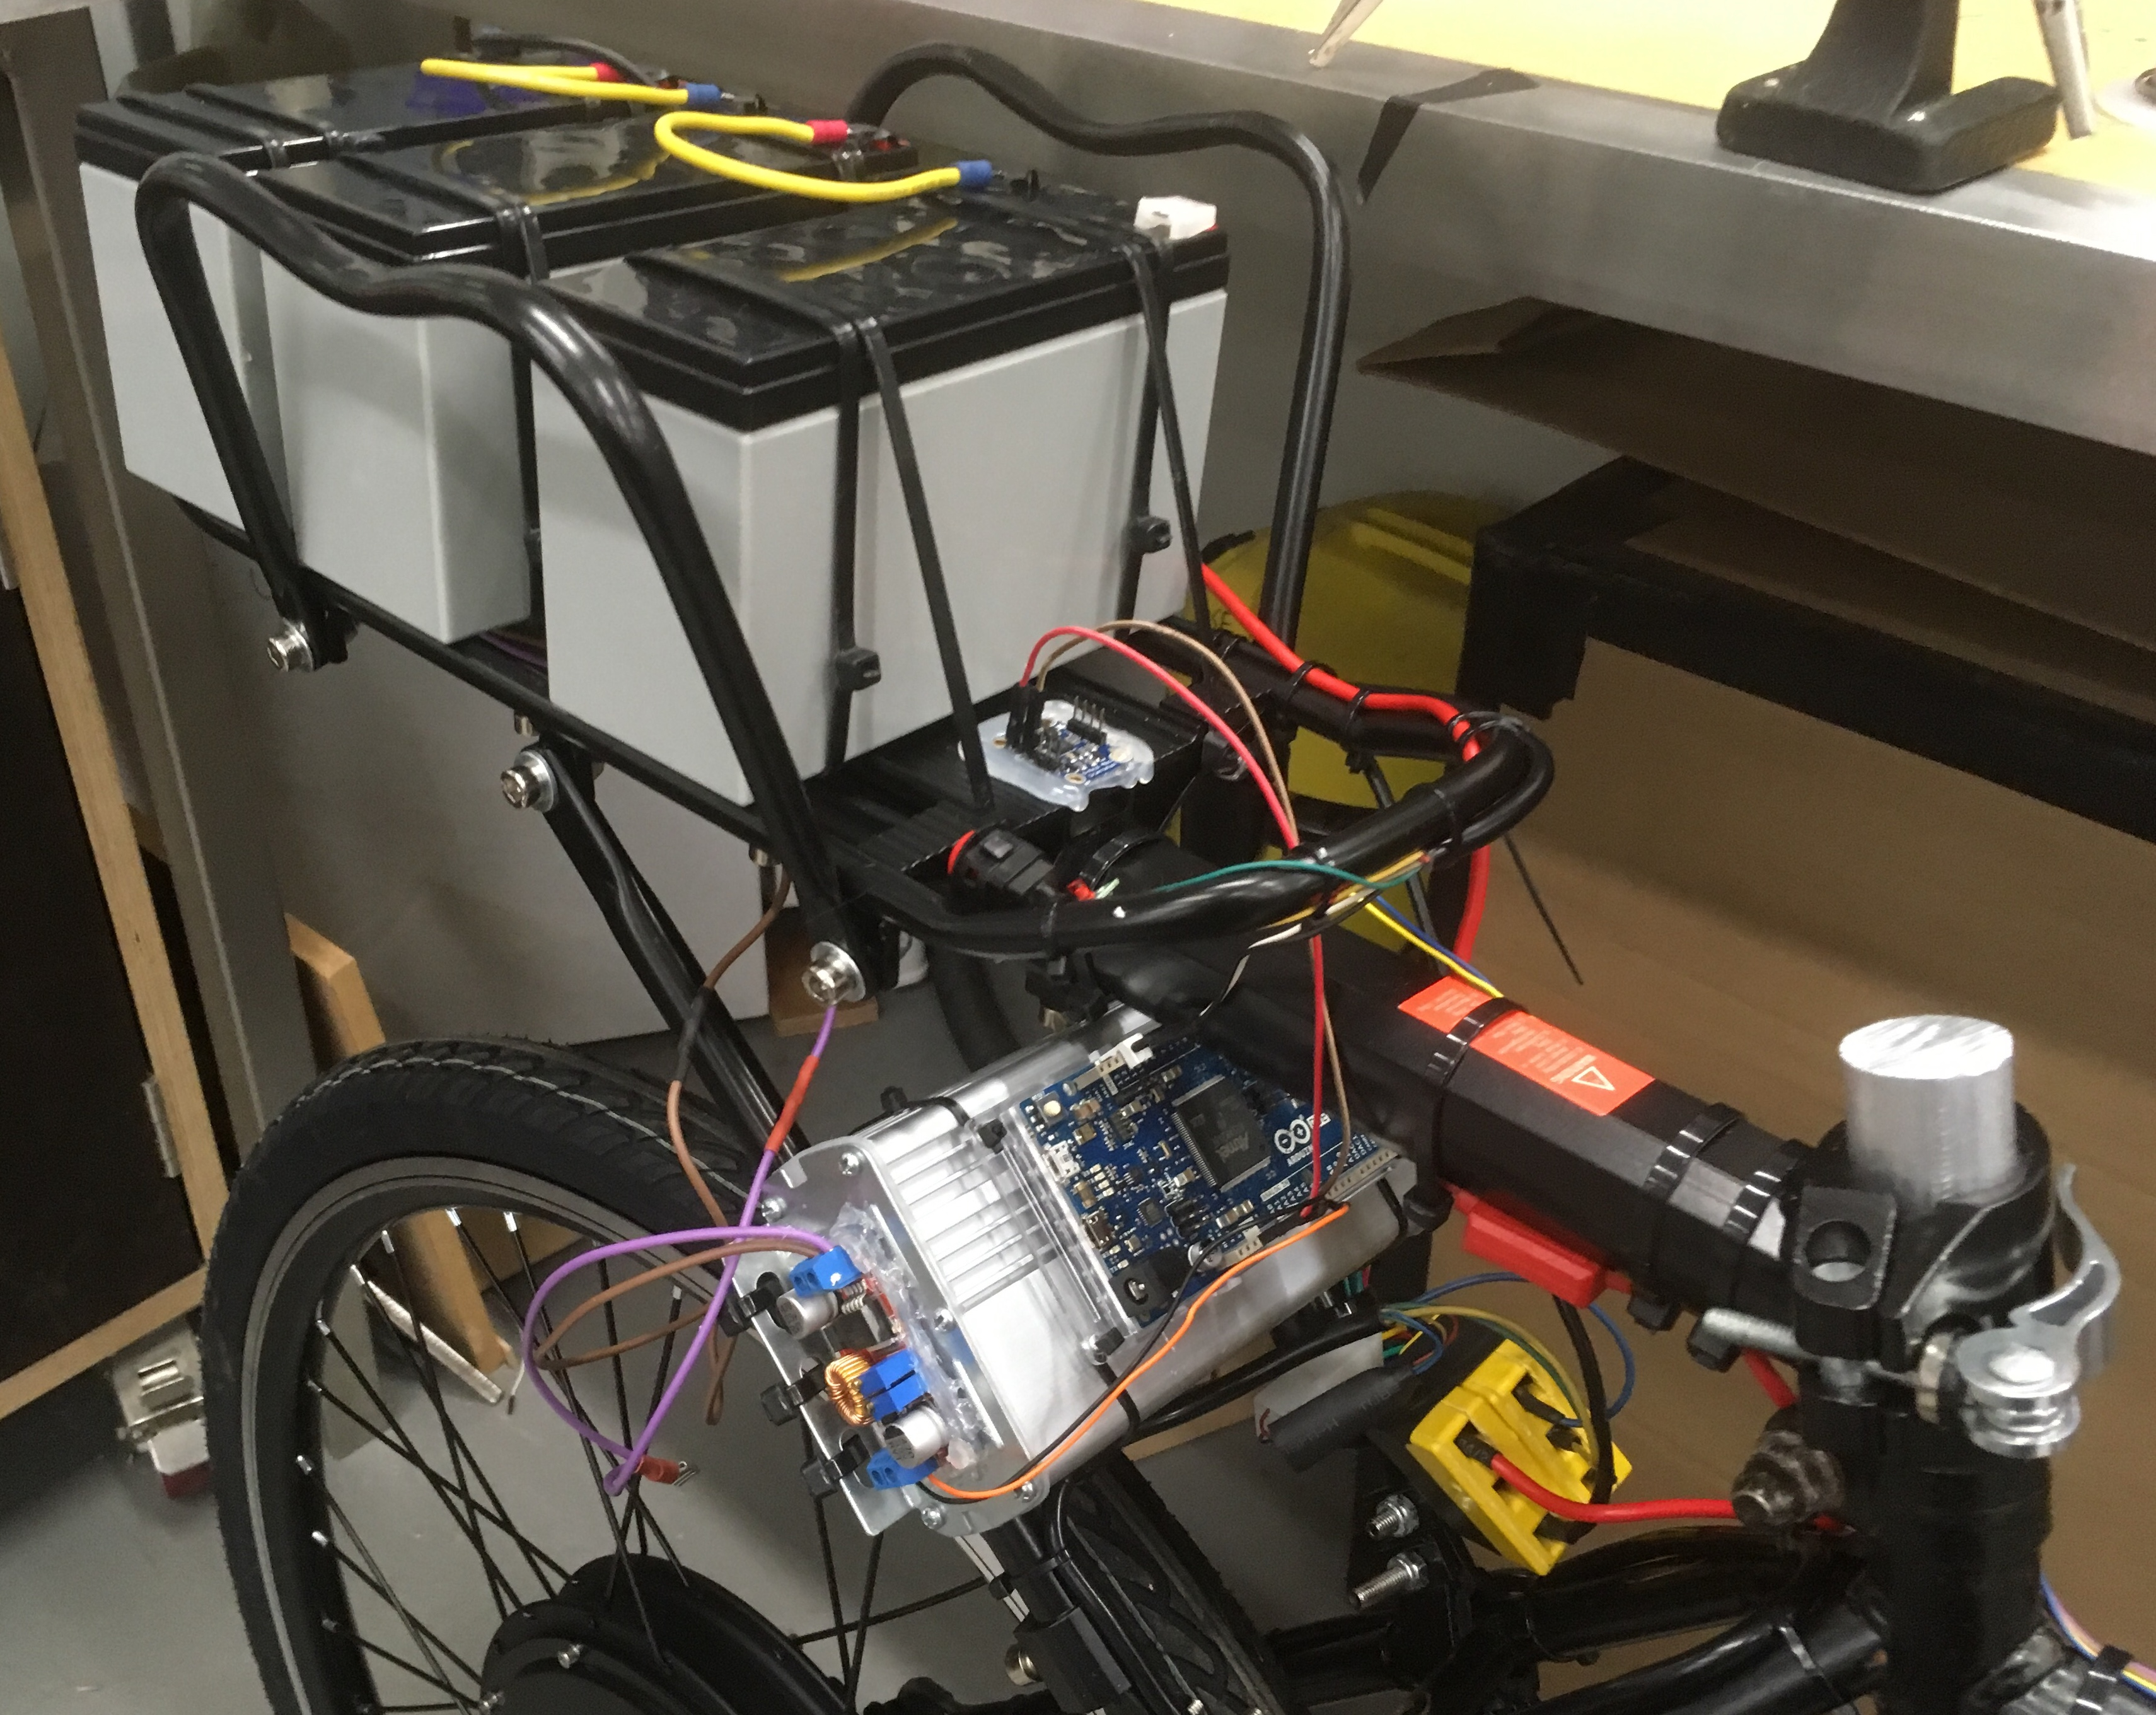
\includegraphics[width=\textwidth]{fsRear}
		\caption{Power and Control Section}
	\end{subfigure}
	\vskip\baselineskip
	\begin{subfigure}[t]{0.475\textwidth}   
		\centering 
		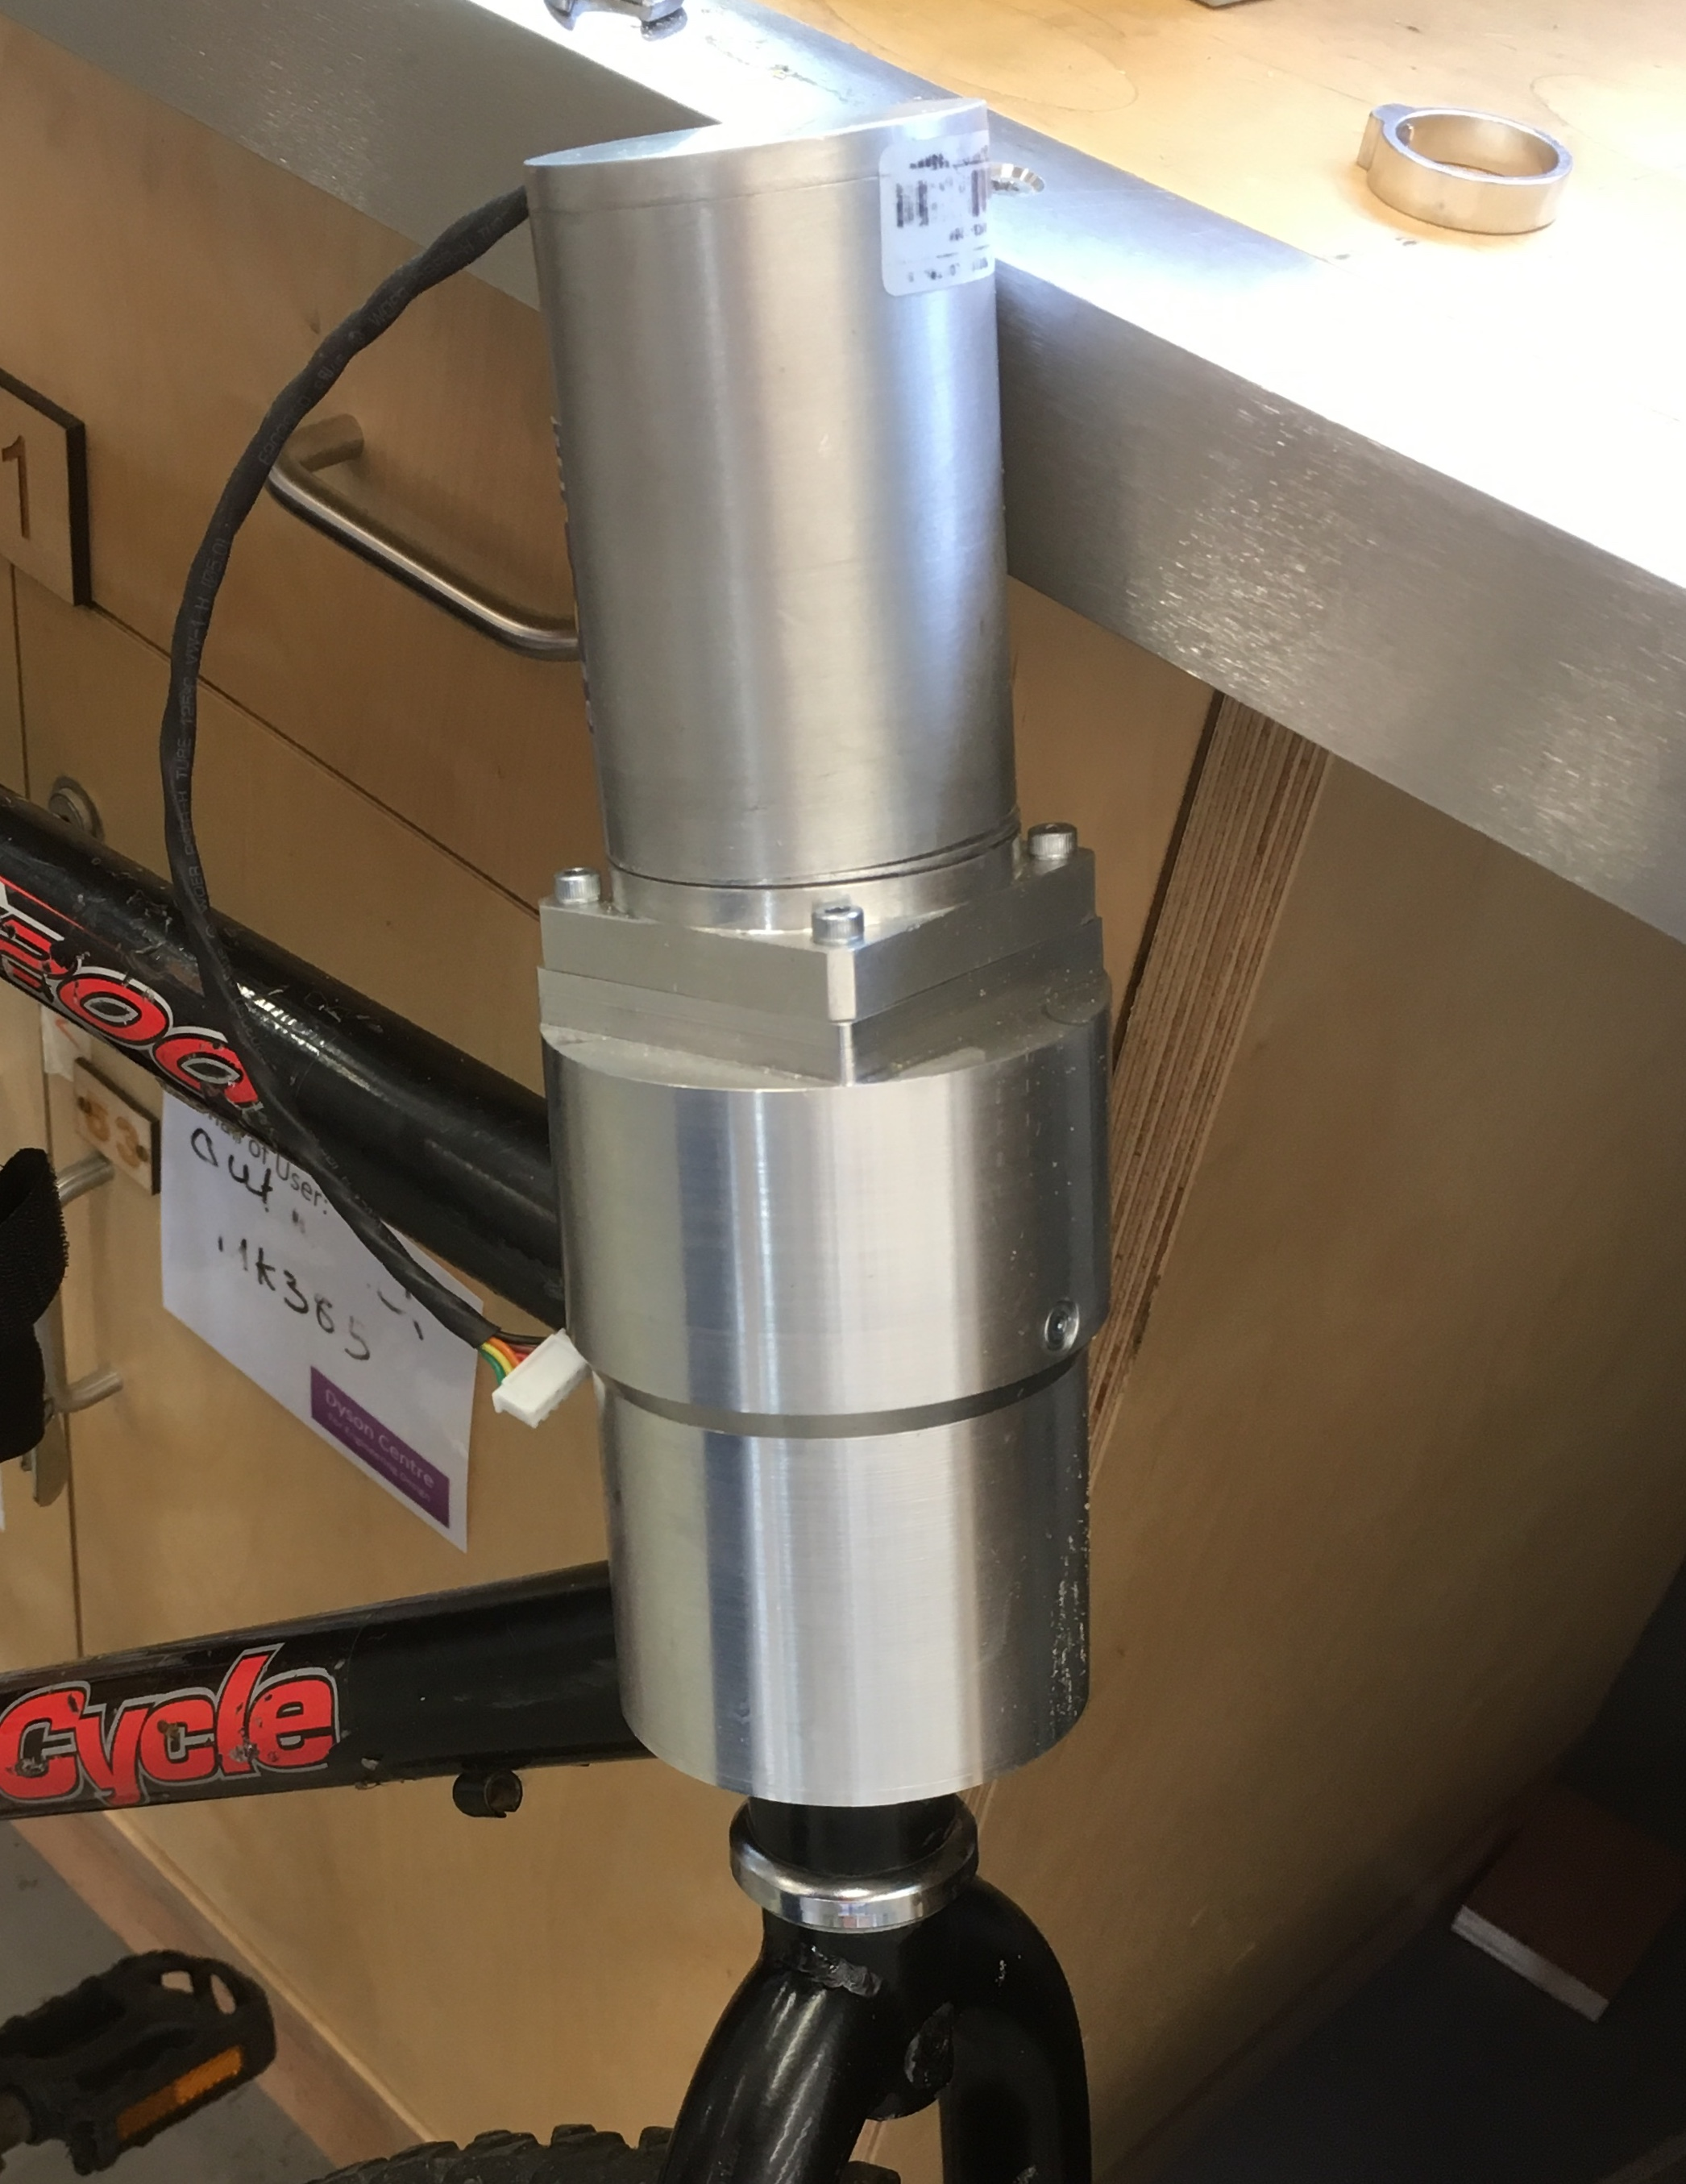
\includegraphics[width=\textwidth]{fsServo}
		\caption{Servo Assembly}
	\end{subfigure}
	\hfill
	\begin{subfigure}[t]{0.475\textwidth}   
		\centering 
		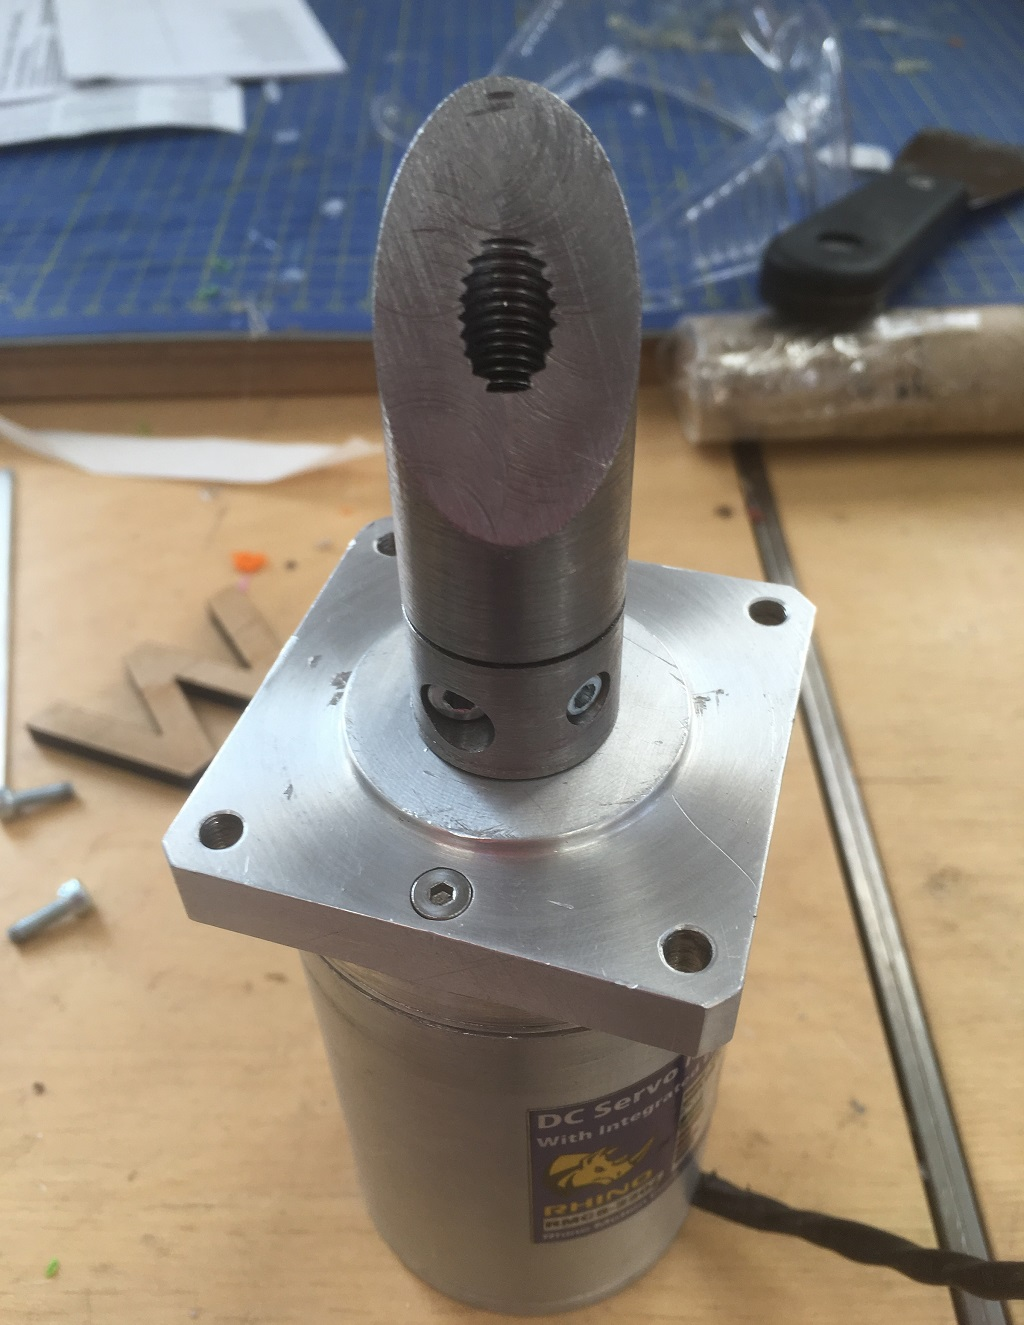
\includegraphics[width=\textwidth]{fsServoMount}
		\caption{Servo Mounting Mechanism}
	\end{subfigure}
	\caption{Full-Scale Bicycle Hardware}
	\label{fig:fsHardware}
\end{figure}

\subsubsection{Microprocessor and Sensors}

\subsubsection{Miscellaneous}

\subsection{Software}

\subsubsection{Code Layout}
Loops at different sample times: IMU, controller, telemetry, etc.

\subsubsection{Lean Angle Estimation}
Again, it was necessary to estimate the lean angle from raw sensor data. In the case of the full-scale bicycle however, an \textit{inertial measurement unit} (IMU) was available, comprised of three gyroscopic sensors and three accelerometers, each aligned along an orthogonal axis. This meant that gyroscopic drift could now be directly accounted for without having to resort to the computationally expensive Kalman filter used for the Lego prototype.\\

At rest, an accelerometer outputs a signal directly proportional to the gravitational vector, this can then be used as a reference to correct for gyroscopic drift. However, when in accelerated motion, the accelerometer output will be \textit{corrupted} by other accelerations terms, such as linear or Coriolis.

The problems present in both accelerometers and gyroscopic sensors are alleviated by the use of a complementary filter. Simply put, an accelerometer is useful over a long duration of time, while a gyroscopic sensors useful over a short period of time. It is therefore possible to low-pass filtere Combining both favourable aspects of these sensors leads to the use of a complementary filter. 

Complementary filter, gyro HPF and acc LPF, more stable since we have accelerometer to correct for drift

\subsubsection{Basestation and Telemetry}

\begin{figure}[h]
\centering
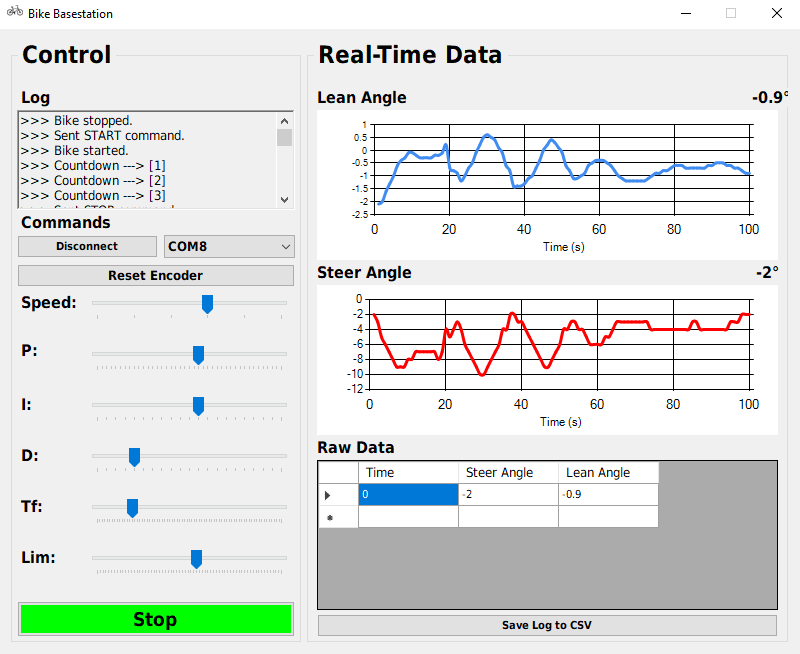
\includegraphics[scale=0.5]{Basestation}
\caption{Screenshot of Bicycle Basestation}
\label{fig:basestation}
\end{figure}

Packet handling, vary controller parameters on the fly, live data logging and display, safety start/stop, etc..

\subsection{Results}